\documentclass{article}
\def\SFunction#1{\textbf{#1()}}
\def\SArg#1{\textsl{#1()}}
\usepackage{times}
\usepackage{fullpage}
%\def\long\question#1{\textit{#1}}
\def\question#1{\textit{#1}}
\usepackage{graphicx}
\usepackage{amsmath}
\author{Duncan Temple Lang}
\title{Approaches for Random Number Generation}
\begin{document}
\maketitle

Statistics attempts to make sense of randomness.  It also uses
randomness in a variety of different ways to perform computations.
Cross-validation involves random permutations of the observations to
create the K-fold test sets.  Similarly, the non-parametric bootstrap
involves sampling with replacement from the observational units.  And
the parametric bootstrap involves sampling from probability
distributions.  R, S-Plus, Matlab and other commonly used software
environments provide functions for for generating random variates from
common probability distributions.  And one is well advised to use
these when they exist as they are likely to be more efficient and
better tested than code that we create ourselves as part of a bigger
project.  In spite of the availability of these common distributions,
we often encounter situations where we need to generate values from a
distribution that is not built-in to these environments.  Generally,
there are several approaches to go about creating samples from these
less common distributions.  One is called the Inverse CDF method.
Another is Acceptance/Rejection sampling.  And a third is Markov Chain
Monte Carlo.

Underlying the computations of all these methods is the ability to
generate pseudo random numbers on a computer. For that we need
suitable random number generators.



\section{Inverse CDF Method}

Suppose we have a random variable $X$ with density function $f_X(x)$
and we want to generate sample values from the corresponding random
variable.  If we can get the inverse function ($F_X^{-1}(x)$) of the
CDF of $X$, then we create a new random variable using the following very
simple procedure:
\begin{itemize}
\item generate a sample, $u$,  from a $U(0, 1)$, i.e. a
 standard Uniform distribution
\item compute $y = F_X^{-1}(u)$.
\end{itemize}
The value $y$ is clearly random since it is based on a random input,
$u$.  And we have a random variable $Y$ defined by this random
procedure.  It turns out that its density is $f_X(x)$, exactly what we
want to sample from. So this procedure generates values from the
random variable $X$ as we set out to do.


It is reasonably easy to verify that the density of our random
variable $Y = F^{-1}(U)$ (where $U ~ U(0,1 )$) is $f_X(x)$, or
equivalently and more readily that the CDF of $Y$ is $F_X(x)$.
\begin{eqnarray*}
 Pr(Y \le x)  &=& Pr(F_X^{-1}(U) < x) \\
  &=& Pr(F_X(F_X^{-1}(U)) < F_X(x)) \\
  &=& Pr(U < F_X(x)) \\
  &=& F_X(x)
\end{eqnarray*}
We use the fact that $F_X$ is monotonically non-increasing and has an
inverse in the step that moves from $Pr(F_X^{-1}(U) < x)$ to the
equivalent $Pr(F_X(F_X^{-1}(U)) < F_X(x))$.  
Also the CDF of a standard uniform is  $F(u) = u$
which follows from integrating the density $f_U(u) = 1$ between
$0$ and $1$.
And the result is simply
that $Y$ has a CDF $F_X(x)$ which is what we wanted to show.

A simpler or more intuitive way to think about why $Y$ has the CDF
$F_X(x)$ is the following.  What we are doing is sampling a percentile
at random when we pick a number $u$ between $0$ and $1$, or $0$ and
$100\%$.
Then we are asking for the corresponding quantile of
the $X$ distribution, i.e. the value $x_u$ of the random
 variable $X$ such that 
 $$F_X( x_u) = u$$ This is easily obtained by using the inverse of
 $F_X$.  So we are matching quantiles of the $U(0, 1)$ distribution
 with the corresponding value in $F_X(x)$.  And by randomly sampling
 the quantiles in $U(0, 1)$, we get random samples from $F_X(x)$.


Since we have the computer at our fingertips, we can verify that the
resulting density is what we expect.  Let's consider a very simple
case, the Exponential distribution.
One parameterization of the density of an Exponential distribution is given as
$$ f_E(x, \lambda) = \frac{1}{\lambda}e^{-x/\lambda}$$ where $\lambda
> 0$ and $x \in (0, \infty)$.
Simple integration gives us the CDF as
$$ F_E(x, \lambda) = 1 - e^{-x/\lambda}$$
The inverse of this function is easy to get.
Let $R$ be $F_E(x, \lambda)$.
Then 
\begin{eqnarray*}
  R &=& 1 - e^{-x/\lambda} \\
  1-R &=& e^{-x/\lambda} \\
  \log(1 - R) &=& -x/\lambda \\
  x &=&  -\lambda \log(1 - R)
\end{eqnarray*}
So 
$$ F^-1_E(x, \lambda) = -\lambda \log(1 - x)$$


% Since we are going to evaluate this at values from a random Uniform,
% we can replace $\log(1 - x)$ with $-\log(x)$ since if $x ~ U(0, 1)$,
% then so is $1 - x ~ U(0, 1)$.

R uses the other parameterization for an Exponential density,
namely
$$ f_E(x) = \alpha e^{- x \alpha}$$ In other words, $\alpha =
1/\lambda$ in the earlier parameterization.  Remembering this, we can
generate a random sample using both the Inverse CDF method and also
from R's built-in \SFunction{rexp} generator.
We will use $\lambda = 4$ and hence $\alpha = .25$.
\begin{verbatim}
u = runif(10000)
x.e = - 4 * log(1 - u)
hist(x.e, prob = TRUE, xlab="X", 
     main = expression(paste("Exponential Distribution: ", lambda == 4)))
curve(dexp(x, .25), 0, max(x.e), add=TRUE, col = "red")
\end{verbatim}

\begin{figure}[htbp]
  \begin{center}
    \leavevmode
     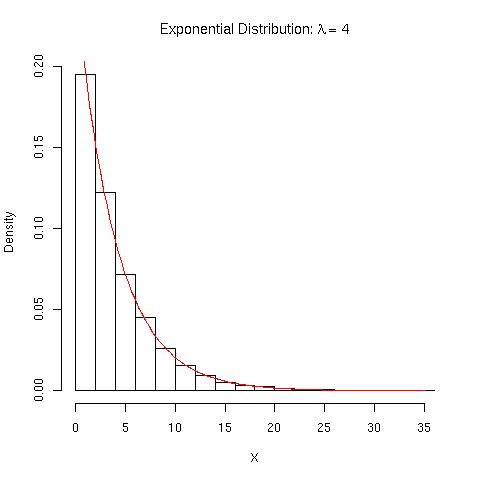
\includegraphics{expInv.jpg}    
    \caption{Sample from an Exponential(4)}
    \label{fig:expInv}
  \end{center}
\end{figure}


We can compare moments of the sample with what we expect.
\begin{verbatim}
> c(mean(x.e), var(x.e))
[1]  3.970798 15.611575
> x.s = rexp(10000, .25)
\end{verbatim}
And we can generate a sample from 
R's built-in generator and compare
the moments.
\begin{verbatim}
> c(mean(x.s), var(x.s))
[1]  3.959364 15.889116
\end{verbatim}
And these agree up to sampling error
with the values $4$ and $16$.

Of course, this simulation does not prove that the inverse CDF method
gives us a random variable with CDF $F_X(x)$.  We needed the math for
that. However, the computer does allow us to explore the technique and
get an understanding of it for particular distributions.

We use the Exponential distribution to illustrate the basics of the
Inverse CDF method. But of course we had the built-in generator
available in R so there was no need.  And, indeed, the generation
technique in R uses a different approach (given by Ahrens and Dieter).
One reason for avoiding the Inverse CDF method is that computing
$F^-1_X(u)$ may be computationally expensive relative to another
approach.  However, the Inverse CDF method is useful when the CDF is
invertible and that inverse function has a reasonably simple form and
there are no built-in functions available to us!  For example, let's
consider a random variable whose distribution is given by the
triangular distribution.  This has a density given
$$
  f_X(x) = 
  \begin{cases}%
   \frac{2(x - a)}{(b-a)(c-a)} & 0 \le x < c, \\
   \frac{2(b -x)}{(b-a)(b-c)} & c \le x \le b \\
   0 & x \not\in [a, b]    
  \end{cases}
$$
and is shown in figure \ref{fig:triangularDensity}.
\begin{figure}[htbp]
  \begin{center}
    \leavevmode
    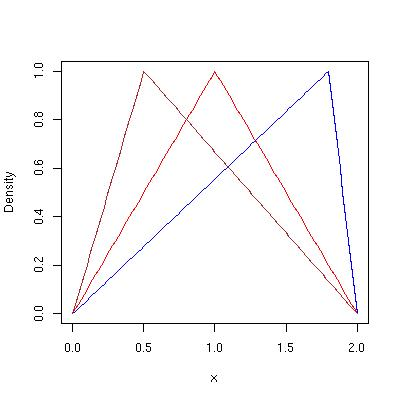
\includegraphics{triangularDensity.jpg}
    \caption{The Triangular Distribution Density.
   These are three different triangular distributions
   on the  interval $[0, 2]$
    with parameters
    $(0, 2, .5)$ (brown), $(0, 2, 1)$ (red), and $(0, 2, 1.8)$ (blue).
   }
    \label{fig:triangularDensity}
  \end{center}
\end{figure}
One can determine these formulae using
the fact that since this is a density, it 
must integrate to $1$. Since we have two triangles
and the area of a triangle is 
$1/2$ base $\times$ height, we get
\begin{eqnarray*}
 1 & = & 1/2 (c-a)\times h + 1/2 (b-c) \times h \\
 2 &=& (b-a) \times h \\
 h &=& 2/(b-a)
\end{eqnarray*}
Then, we have the two points on each line
and we can use the formula for a line.


We can integrate the two components
in the density to get the CDF.
This yields
$$
  F_X(x) = 
  \begin{cases}
  \frac{(x - a)^2}{(b-a)(c-a)} & 0 \le x < c\\
                  1 - \frac{(b -x)^2}{(b-a)(b-c)} & c \le x \le b \\
                  0 & x < 0 \\
                  1 & x > b
  \end{cases}
$$

And finally, we must compute the inverse.  Unlike the case of the
exponential distribution, we have a quadratic function here and we
have two roots.
Taking the case where $c \le x < b$, we have
\begin{eqnarray*}
  R = 1 - \frac{(b-x)^2}{(b-a)(b-c)} \\
  (1 - R)(b-a)(b-c) = (b-x)^2 \\
  \sqrt{(1 - R)(b-a)(b-c)} = b - x \\
\end{eqnarray*}
We can ignore the other root which is $-\sqrt{(1 - R)(b-a)(b-c)}$
because $b - x$ must be positive as $x \le b$ and also $R < 1$ since
it is our uniform random number.  We can similarly invert the other
term in the CDF.  All that is left is that we need to determine the
intervals for which these two pieces in the inverse CDF apply.  The
splitting point on the X axis is $c$.  However, we need this on the
uniform - $[0,1]$ - scale.  The breakpoint on this scale is the
probability or area under the CDF up to the point $c$.
In other words, it is the area of the left triangle in 
the distribution. And this is
$1/2 (c-a) h$  = $(c-a)/(b-a)$. So the 
inverse of the CDF is 
$$
  F^{-1}_X(x) =
  \begin{cases}
    \sqrt{x(b-a)(c-a)} + a &  0 \le x < (c-a)/(b-a)\\
    b - \sqrt{(1 - x)(b-a)(b-c)} & (c-a)/(b-a) \le x \le 1 \\
    0 & x < 0 \\
    1 & x > b
  \end{cases}
$$

And now we can generate random numbers from a Triangular
distribution with parameters $(a, b, c)$ with $(a \le c \le b)$
using the R function
\begin{verbatim}
rtriang =
function(n, a = 0, b = 2, c = 1) {

    if(!(a <= c && c <= b))
      stop("Incorrect parameters")

    x = runif(n)

    ans = rep(0, length(x))
    ans[x > b] = NA

    cutPoint = (c-a)/(b-a)
    A = (x > a & x < cutPoint)
    B = (x >= cutPoint & x <= b)

    ans[A] = sqrt(x[A]*(b-a)*(c-a)) + a
    ans[B] = b - sqrt((1-x[B])*(b-a)*(b-c)) 

    ans
}
\end{verbatim}

Now we can generate our samples and compare the
result
\begin{verbatim}
x = rtriang(10000, 0, 3, 1)
hist(x, prob = TRUE, xlab= "X", main = "Triangular(0, 3, 1)")
curve(dtriang(x, 0, 3, 1), 0, 3, add = TRUE, col = "red")
\end{verbatim}
And, of course,  we get very good agreement with 
the only difference being sampling variability.


\subsection{Distributions}
There are several common distributions that are amenable to the
Inverse CDF method.  We have seen the triangular and exponential
distributions.  The Extreme value, geometric, logistic, Pareto and
Weibull distributions can also be handled in this way.
The Extreme value distribution has density and CDF given
by
\begin{eqnarray*}
f_{\hbox{Extreme Value}}(x) &=& \frac{1}{\beta}e^\frac{x-\mu}{\beta}e^{-e^{\frac{x-\mu}{\beta}}} \\
F_{\hbox{Extreme Value}}(x) &=& 1 - e^{e^\frac{x - \mu}{\beta}}  
\end{eqnarray*}

The CDF of the Geometric is
\begin{equation}
  F_{\hbox{Geo}}(x) = 1 - (1-p)^x
\end{equation}


The CDF of the Logistic is
\begin{equation}
  F_{\hbox{Logistic}}(x) = 1 - 1/(1 + e^{(x - \mu)/b})
\end{equation}

The CDF of the Pareto is
\begin{equation}
  F_{\hbox{Pareto}}(x) = 1 - x^a
\end{equation}

And the CDF of the Weibull is
\begin{equation}
  F_{\hbox{Weibull}}(x) = 1 - e^{(x/a)^b}
\end{equation}



\section{Rejection/Acceptance Sampling}
The Inverse CDF approach works well if a) we can obtain a formula for
the inverse CDF, b) evaluating the formula for a given $u$ is not
excessively expensive.  If we have a density function $f_X(x)$ and we
cannot get the inverse of its CDF, then we are stuck.  How can we
generate random values from that density?  Jon Von Neumann, the
``father of computer architecture'', devised a procedure that allows
us to create samples from essentially arbitrary density functions,
$f_X(x)$.  The idea is quite simple and intuitive.  Let's focus on a
particular density, say the $\beta(4, 3)$.  This is
shown in figure \ref{fig:beta43}.
\begin{figure}[htbp]
  \begin{center}
    \leavevmode
    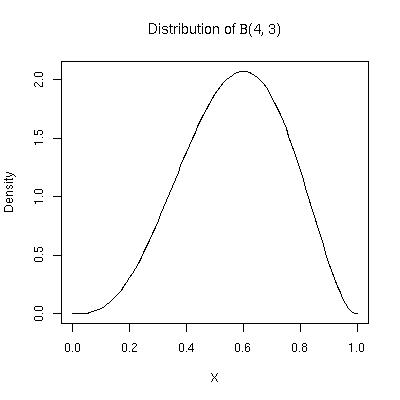
\includegraphics{beta43.jpg}
    \caption{Beta distribution - $\beta(4, 3)$}
    \label{fig:beta43}
  \end{center}
\end{figure}
What we really want to do is sample uniformly from the region under
this density.  If we could throw an infinite number of darts at the
2-dimensional plane $\Re \times \Re$ in a random way, then we could
consider only the darts that were within the region described by the
density.  Then we could take the $X$ coordinate of each of those darts
and that would constitute a random sample.  And these values would
have the appropriate density $f_X(x)$.  You should convince yourselves
that they do have the desired density.

Now, there are two problems with this approach.  We have to throw a
lot of darts!  This is time consuming and perhaps dangerous.  And if
we really throw them at random onto the entire plane, we will waste an
enormous amount of them.  Specifically, a relatively small proportion
will actually end up under the density.  After all, we are only
looking for values under the curve that ranges from $0$ to $1$ on the
X axis and from $0$ to $2.08$ on the Y axis. (\question{How can we
  determine this value?}).  What we are looking for is a more
efficient mechanism that we can use on a computer.

If we really could throw darts, we would try to narrow down the area
at which we are throwing them so that we wouldn't waste as many.
Suppose we consider the rectangle that encloses this entire density,
namely the Cartesian region $[0,1] \times [0, 2.08]$
shown in figure \ref{fig:beta43Unif}
\begin{figure}[htbp]
  \begin{center}
    \leavevmode
    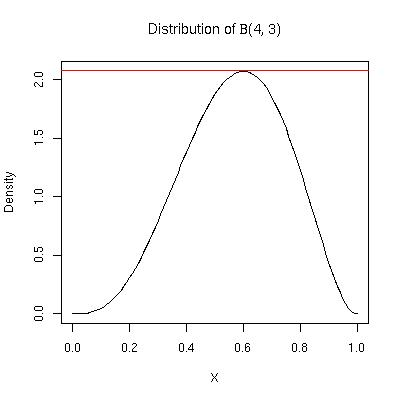
\includegraphics{beta43Unif.jpg}
    \caption{Envelope of the $\beta(4, 3)$ density.}
    \label{fig:beta43Unif}
  \end{center}
\end{figure}
If we could throw darts only in this region, then many more would be
actually ``accepted'' in our sample, i.e. be within the region under
the density.

This is the basic idea.  We try to sample uniformly from under the
density, but we cannot do this easily.  So we try to sample uniformly
from a bigger region that encloses the area of interest (our density)
and then we take only the samples within our area of interest.  If we
agree that this is a strategy that would yield a sample with the
correct distribution, i.e. with a density $f_X(x)$ then we have only
one thing left to figure out.  And that is how can we do this
practically and on a computer?

The answer involves a two-step random procedure.  We have to sample
the larger region that encloses our density.  Unlike our other random
number generation techniques, this involves sampling from a $2$
dimensional region.  So we want to avoid this if possible.  What we
will do is quite clever, thanks to John Von Neumann.  We break this
into two $1$ dimensional sampling steps.  What we do is to find a
random variable that we can sample from.  Ideally, it would have the
same \textit{support} (i.e. range) as the random variable of actual
interest (i.e the on with density $f_X(x)$).  Then, we generate a
second value that gives us the second dimension.  And this allows us
to sample uniformly in the larger region. And then we do our
``rejection-acceptance'' trick by checking whether the point is inside
the region in which we are actually interested. 

We have described this procedure in words. At some point we have to
put this into technical terms so that we can use it on the computer.
And we will also need to write it mathematically so that we can prove
that the resulting random procedure creates random values with the
correct density.  So now is a good time.  Let's suppose we can find a
second probability density function, $g_Y(y)$ that we can sample from.
Obviously, this must integrate to $1$. So its area is the same as the
density in which we are interested, $f_X(x)$.  So we know that the
density $g_Y()$ cannot entirely contain $f_X(x)$.  However, what if we
could multiply this density $g_X(x)$ by some number $c$
so that 
$$ c \times g_Y(x) \ge f_X(x) \forall x.$$ If this is possible, then
we can do the following.  Generate a random value from the density
$g_Y()$, say $y$.  Then, generate a value ($u$) from a Uniform
distribution between $0$ and $c g_Y(y)$.  We accept $y$ as being a
value in our target sample if $u < f_X(y)$.
In other words, if $u$ is within the region enclosed by $f_X(x)$,
we keep it; otherwise we reject it and return to the original
sampling steps.

So the acceptance/rejection sampling procedure in more algorithmic
terms is as follows:
\begin{enumerate}
\item Select $g_Y(y)$ and $c$ such that  
    $c g_Y(x) > f(x) \forall x$ of interest.
\item Generate a random value, $y$,  from $g_Y()$.
\item Generate a random value, $u$, from $U(0, c g_Y(y))$.
\item Accept $y$ if $u \le f_X(y)$.
  Otherwise, return to step $2$.
\end{enumerate}


Let's return to our example of the $\beta(4, 3)$.  One of the simplest
choices for $g_Y()$ is the uniform distribution.  It is especially
simple in this case as the $\beta(\cdot, \cdot)$ distribution has
support on the interval $[0, 1]$, just like $U(0, 1)$.  We then need
to select $c$ so that the density $c$ times the density $g_Y(y) = 1$
is greater than the density of the $\beta(4, 3)$.  We can eyeball this
by plotting the density $f_X(x)$ and taking a sufficiently large value
of $c$.  From figure \ref{fig:beta43Unif}, we see that anything above
$\approx 2.1$ is fine. So $2.5$ will work to be on the safe side.

What happens if we chose $c$ conservatively?  We are enlarging the
region in which we take our potential sample of values.  The larger
this is relative to the region under the density $f_X(x)$, the greater
the number of samples that will be rejected.  As a result, we will
have to generate more potential samples if we need to get a fixed
number $n$ accepted samples.  So choosing our enveloping region as
close as possible to the region of interest (i.e. under $f_X(x)$) is
highly desirable. When using the Uniform distribution, i.e. a
rectangular enveloping region, we want to chose $c$ to be the maximum
of our density $f_X(x)$.  A little calculus allows us to find this.
Alternatively, we can use R to obtain an approximate answer
by evaluating the density at different points 
\begin{verbatim}
 max(dbeta(seq(0, 1, length = 100000), 4, 3)
\end{verbatim}
yielding $2.07$.


So now we are set to perform the different steps to generate a value
from a $\beta(4, 3)$ random variable.
\begin{verbatim}
 while(TRUE) {
   y = runif(1)
   u = runif(1, max = 2.07 * y)
   if(u < dbeta(y, 4, 3))
     break
}
\end{verbatim}

I have written some functions that allow us to explore different
choices of $g_Y()$ and to generate samples.
Using a simple rectangular sampling region
via the standard Uniform density for $g_Y()$,
we get
\begin{figure}[htbp]
  \begin{center}
    \leavevmode
    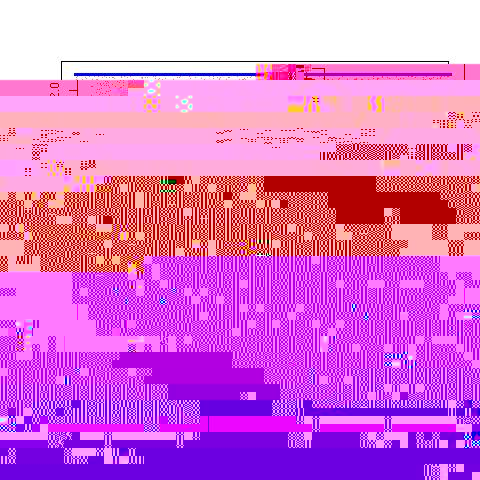
\includegraphics{ARSBetaUnif.jpg}
    \caption{Acceptance/Rejection using the triangular distribution}
    \label{fig:betaUnif.jpg}
  \end{center}
\end{figure}
The proportion of samples that were accepted is $47.3\%$.
We see that the sample histogram is very close to the
density and the variation is just sampling error.

By choosing a better enveloping region, we can improve the acceptance
rate.  In the case of the $\beta(4,3)$ density, we can use a
triangular distribution as $g_Y()$ and scale it to create an envelope
region. The particular choice of triangular distribution is $Tr(0, 1,
.8)$ and we choose $c$ to be $1.6$.  The plot in figure
\ref{fig:betaTriang.jpg} shows this region.
\begin{verbatim}
acc = ars.eg(function(x) dbeta(x, 4,3), 
             function(x) dtriang(x, 0, 1, .8), 
             1.6, 
             function(n) tr.inv(runif(n), 0, 1, .8), 
             10000)
\end{verbatim}
\begin{figure}[htbp]
  \begin{center}
    \leavevmode
    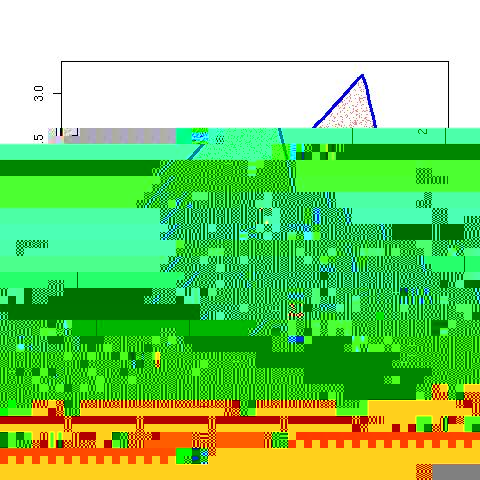
\includegraphics{ARSBetaTriangular.jpg}
    \caption{Acceptance/Rejection using the triangular distribution}
    \label{fig:betaTriang.jpg}
  \end{center}
\end{figure}
The acceptance rate for this is $62\%$.


\section{Markov Chain Monte Carlo - MCMC}
In most simulation contexts, we are interested in estimating the
expression $E_{f_X}[g(X)]$.
If we have i.i.d. samples from the random variable with density $f_X$
of the form $x_1, \ldots, x_n$, we can estimate this value
as
\begin{equation}\label{egx}
 E_{f_X}[g(X)] \approx \frac{1}{n} \Sigma_{i=1}^n g(x_i)
\end{equation}
The law of large numbers tells us that this is a good estimator.
Using different functions $g()$, we can obtain estimates for different
properties.  For example, $g(x) = x$ gives us the expectation of the
random variable.


Identical and independent values may be hard to sample from $f_X(x)$.
But we can use the estimator above in \ref{egx} if the $x_i$ are not
independent but sampled from $f_X(x)$ in proportion to $f_X()$.  The
computation of the variance is more complicated in these
circumstances, but the estimator is good.  This is because
\begin{equation}
  E_{f_X}[g(x)] = \int g(x) f_X(x) dx
\end{equation}
So if we can generate $x_i$ from $f_X()$ we can use Monte Carlo to
solve many problems.

The problem that we are now faced with is how to generate sample
values from the density $f_X(x)$, dependent or independent.  It turns
out that this is actually quite simple if we use what are called
Markov Chains.  Consider the following technique for generating a
sequence of random values.  Define $X_{t+1}$ by sampling from a
distribution that only depends on $X_t$, i.e. the current state of the
sequence.  In other words, we have a probability distribution given in
general terms as $P(X_{t+1} \vert X_t)$.  This sequence ${X_t}$ is
called a Markov chain.

To get the sequence started, we need a starting value $X_0$.  But
$X_{t}$ will depend on the value of $X_0$.  For many probability
distributions $P(X_{t+1} | X_t)$, it turns out that $P(. | X_0)$ is
independent of $X_0$ and it doesn't matter where we start.  And under
certain conditions, the sequence ${X_t}$ converges to a stationary
distribution, $\pi(x)$, which does not depend on $t$ or $X_0$.  Thus
for a sufficiently large value of $t$, $t_0$, $X_{t_{0} + 1}, X_{t_{0}
  + 2}, \ldots$ are samples (\textit{not} necessarily independent)
from the density $\pi(x)$.
So we can estimate $E_{g_X}[X]$ as 
\begin{equation}
  \frac{1}{n - t_0}\Sigma_{i = t_0}^n g(x_i)
\end{equation}


All that remains to use this technique is to create the Markov Chain.
In other words, we must specify the value $P(X_{t+1} \vert X_t)$ so
that we obtain the desired stationary distribution $f_X(x)$.  This
seems like a hard task, but it turns out to be quite simple.  Suppose
we have a distribution function $q(\cdot \vert X_t)$ which we will
call our \textit{proposal} distribution.  For a given $t$, we generate
a sample from a random variable $Y$ with this density.  We call $q()$
a proposal distribution because we don't use it directly to generate
$X_{t+1}$ in our sequence. Instead, we generate this new value but,
like acceptance/rejection sampling, we decide whether to accept it
under certain conditions.  Specifically, we use an decision algorithm
to accept or reject this new value.
The Hastings algorithm decides to accept this new value
with probability
$$
 min(1, \frac{f_X(Y)}{f_X(X_t)})
 $$ In other words, we toss a weighted coin with probability $ min(1,
 \frac{f_X(Y)}{f_X(X_t)})$ and if it turns up heads, we accept the new
 value $Y$ as the next step in the sequence, $X_{t+1}$.  If the coin
 ends up tails, we stay where we are and $X_{t+1} = X_t$.  This
 acceptance probability essentially favors $Y$ if $Y$ is more likely
 than the current value $X_{t}$.

The Metropolis-Hastings algorithm adds a variation to this.
Instead of looking at the likelihood ratio of $f_X(Y)/f_X(X_t)$,
it uses
$$
 \frac{q(X\vert Y) f_X(Y)}{q(Y\vert X) f_X(X)}
 $$ 
where $q$ is our proposal distribution again.
This yields nice properties that allow the Markov Chain to be
reversible and generally nicely behaved.

Regardless of which algorithm we use to accept or reject or our
proposal $Y$, the algorithm for generating the steps in the Markov
Chain are quite simple.

We need a function to generate a value from our proposal distribution.
This is the argument \SArg{r}.  To compute the acceptance probability,
we need $f_X()$, the stationary target density.  And if we are using
the Metropolis-Hastings algorithm we also need the density of the
proposal distribution given by \SArg{q}.  And we need a starting
point, $X_0$.  \SArg{n} says how many elements in the sequence we
should generate.  We need this to be large enough so that the chain
converges to $f_X()$ and yields sufficient sample values.
\begin{verbatim}
mcmc =
function(x.0 = 0, r, q, stationary, n = 1000, algorithm = metropolis)
{
     xs = numeric(n+1)  # space for the answers
     xs[1] = x.0
     for(i in 1:n) {
       y = r(xs[i])   # Generate proposal
       k = algorithm(xs[i], y, stationary, q)
       xs[i+1] = ifelse(runif(1) <= k, y, xs[i])
       if(is.na(xs[i+1])) {
        stop("Problems in MCMC")
       }
     }

     class(xs) <- "mcmc"
     xs
}
\end{verbatim}

Let's generate a sample from a t-distribution with $10$ degrees of
freedom, $t(10)$.  This is the stationary distribution that is our
target.  We can use the R function \SFunction{dt} to compute the
density.  We will use a Normal distribution as our proposal
distribution with mean $X_t$ and variance $1$.  We can use
\SFunction{rnorm} to generate proposal values and \SFunction{dnorm} to
calculate the density in the Hastings algorithm.
We'll generate $10,000$ values and then look at the last
$5000$ to give this adequate time to ``burn in'' or converge
to $t(10)$. We'll chose a strange starting value of $-10$
to illustrate how this converges.
\begin{verbatim}
 xt = mcmc(-10, 
           r = function(x) rnorm(1, x), 
           q = function(x, y) dnorm(y, x), 
           stationary = function(x) dt(x, 10), 
           alg = hastings, 
           n = 10000)
\end{verbatim}
We can see how well the sample approximates the
true density $t(10)$ in figure
\begin{figure}[htbp]
  \begin{center}
    \leavevmode
    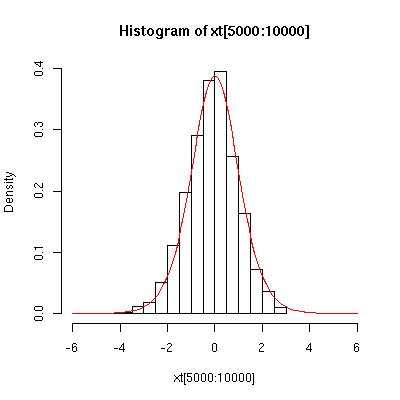
\includegraphics{mcmcT10.jpg}
    \caption{MCMC sample from $t(10)$.}
    \label{fig:mcmcT10.jpg}
  \end{center}
\end{figure}
This looks pretty close and within sampling variation.


The MCMC  approach to estimating $E[g(X)]$ and sampling dependent
values from a density is very powerful and is similar in ways to the
acceptance/rejection sampling we covered above.  One does have to
honor the conditions on the proposal and stationary distributions to
ensure that the Markov chain converges and converges to $f_X()$.


\end{document}

